\documentclass[a4paper,12pt]{article}

\usepackage[utf8]{inputenc}
\usepackage[T1]{fontenc}
\usepackage[english, german]{babel}
\usepackage{fancyhdr} %Kopf und Fußzeile
\usepackage{graphicx}
\usepackage{enumitem}
\usepackage{calc} 
\usepackage{caption}

\usepackage{amsmath}
\usepackage[backend=biber, style=apa]{biblatex} % BibLaTeX-Paket
\addbibresource{expose.bib} % Pfad zur Bibliografiedatei
\graphicspath{{./bilder/}{./}}

% use last
\usepackage{xurl} % URL-Zeilenumbruch
\usepackage[colorlinks=true,allcolors=black]{hyperref}

\usepackage{float} %Bilder an bestimmter Stelle platzieren


\setlength{\parindent}{0pt} % cm, mm, in
\setlength{\parskip}{0.6ex plus 0.3ex minus 0.2ex} %elastisches Maß, um unschöne Seitenumbrüche zu vermeiden

% Kopf und Fußzeilen
\pagestyle{fancy}
\lhead{
\includegraphics[height=3ex]{FomLogo}}
\rhead{\thepage}
\lfoot{2023-09-19}
\cfoot{}

\begin{document}

% !TeX root = main.tex
\begin{titlepage}

	\centering
	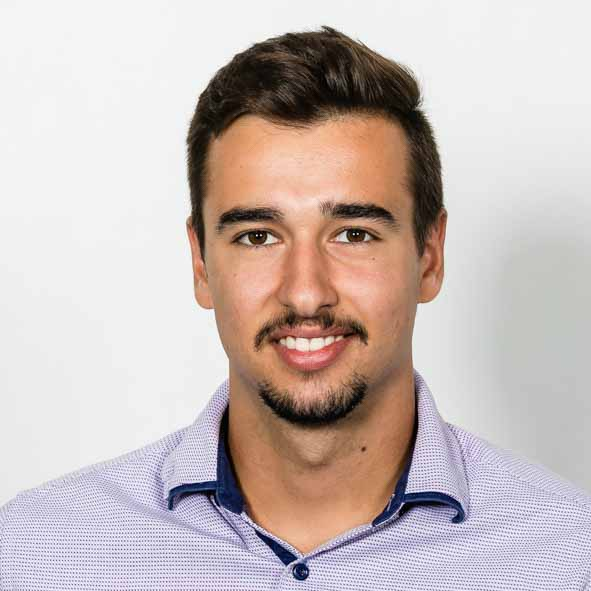
\includegraphics[width=0.15\textwidth]{ASadowski}\par\vspace{1cm}
	{\scshape\LARGE FOM - Hochschule für Oekonomie und Management \par}
	\vspace{1cm}
	{\scshape\Large Bachelor Arbeit\par}
	\vspace{1.5cm}
	{\huge\bfseries Die sehr spannende akademisch wissenschaftliche Arbeit\par}
	\vspace{2cm}
	{\Large\itshape Alexander Sadowski\par}
	\vfill
	supervised by\par
	Dr.~Mark \textsc{Brown}

	\vfill

% Bottom of the page
	{\large \today\par}
\end{titlepage}
\pagenumbering{Roman}

\newpage
\tableofcontents

\newpage
\listoffigures %Abbildungsverzeichnis

\newpage
\listoftables

\newpage
% !TeX root=main.tex


\section *{Abkürzungsverzeichnis} % das Sternchen * sorgt dafür, dass die Section nicht nummeriert wird und nicht im Inhaltsverzeichnis auftaucht
\begin{description}
    \item[AI:] Artificial Intelligence
    \item[BI:] Business Intelligence
    \item[DSR:] Design Science Research
    \item[KI:] Künstliche Intelligenz
    \item[LLM:] Large Language Models
    \item[NLP:] Natural Language Processing
\end{description}


\newpage
\pagenumbering{arabic}
\thispagestyle{empty} %keine Kopf und Fußzeile oder {plain}

% !TeX root = main.tex

\section{Einleitung} 
\label{sec:einleitung}

Die Studie von Dwivedi et al.\footnote{Vgl. \cite{DwivediHughes2021}, S.11-13} beschreibt KI als eine transformative Technologie, die menschliche Aufgaben und Aktivitäten in vielen Bereichen ergänzen oder ersetzen kann. Ein besonders vielversprechender Aspekt in diesem Bereich ist die Anwendung von Large Language Models (LLM) in Business Intelligence (BI)-Lösungen. Diese Integration zielt darauf ab, Arbeitsabläufe zu rationalisieren, menschliche Fehler zu reduzieren und datengesteuerte Entscheidungsprozesse zu ermöglichen. 
Die Einzelhandelsbranche, insbesondere der Schuhsektor, bietet vielseitige Gelegenheiten, diese Vorteile zu nutzen. Manuelle Prozesse im Einzelhandel, wie z. B. Bestandsverwaltung, Kundenservice und Verkaufsanalyse, sind oft zeitaufwändig und fehleranfällig.\footnote{Vgl. \cite{Perez2018}, S.1-10; \cite{Lee2018}, S.20} Durch den Einsatz von LLM in BI-Lösungen könnten diesen Aufgaben automatisiert werden, so dass Einblicke in Echtzeit möglich sind und sich die Mitarbeiter auf strategischere Tätigkeiten konzentrieren können.


Mit der Veröffentlichung des LLM GPT-3 im Jahr 2020 hat OpenAI einen Meilenstein in der KI-Forschung gesetzt. GPT-3 ist ein Sprachmodell, das auf der Grundlage von 175 Milliarden Parametern trainiert wurde und in der Lage ist, menschenähnliche Texte zu generieren.\footnote{Vgl. \cite{Brown2020}, S.2} Das LLM hat das Potenzial, die Art und Weise, wie wir mit Computern interagieren, zu revolutionieren und die KI-Technologie auf ein neues Niveau zu heben.\footnote{Vgl. \cite{Lu2021}, S.1046-1047} OpenAI hat das Modell als Chatbot kostenlos und für jedermann zugänglich gemacht, wodurch die KI-Technologie in die Gesellschaft eingeführt wurde. Erste Studien haben das Potenzial von LLM für die Umgestaltung von Geschäftsprozessen aufgezeigt. So kann laut einer Studie von Prabhavathi et al.\footnote{Vgl. \cite{Prabhavathi2019}, S.161-162} die Integration von LLM im Einzelhandel das Kundenerlebnis durch die Automatisierung von Abfrageantworten und die Bereitstellung personalisierter Empfehlungen erheblich verbessern. In ähnlicher Weise zeigten Ibrahima et. al.\footnote{Vgl. \cite{Ibrahima2021}, S.33}, wie LLM-gestützte BI-Lösungen, die Genauigkeit der Bestandsverwaltung durch die Analyse von Verkaufsmustern und die Vorhersage des Lagerbedarfs verbessern können.

Jüngste Fortschritte unterstreichen die Relevanz dieser Integration weiter. Die Entwicklung von Tools wie Microsofts Copilot für Microsoft 365 zeigt die praktische Anwendung von LLMs bei der Automatisierung von Routineaufgaben und der Steigerung der Produktivität im Unternehmenskontext. Das Microsoft Copilot-System nutzt LLMs, um Benutzer bei der Erstellung von Inhalten, der Analyse von Daten und der Automatisierung sich wiederholender Aufgaben zu unterstützen und so den manuellen Aufwand in BI-Prozessen erheblich zu reduzieren.\footnote{Vgl. \cite{Spataro2024}, S.1-7}

Die Relevanz dieses Themas wird durch die steigende Nachfrage nach effizienten Datenmanagement- und Analysewerkzeugen in der heutigen datengesteuerten Geschäftsumgebung unterstrichen.\footnote{Vgl. \cite{Syam2018}, S.135-136} Durch die Untersuchung des Potenzials von LLMs innerhalb von BI-Lösungen soll diese Arbeit einen Einblick geben, wie diese fortschrittlichen Technologien genutzt werden können, um Geschäftsprozesse zu automatisieren und zu optimieren.

\newpage

% !TeX root=main.tex

\section{Arbeitstitel}

\subsection{Fundamentales}
Am Anfang war das Wort, siehe~\ref{sec:ziel}%es wird Bezug


\clearpage
% !TeX root=main.tex

\section{Forschungsfragen und Ziel der Arbeit}

Die zentrale Forschungsfrage dieser Bachelorthesis lautet:

\begin{description}
    \item[MRQ:] ''Wie können LLMs innerhalb des BI-Kontexts genutzt werden, um manuelle Prozesse zu automatisieren, und welche Auswirkungen hat dies auf Effizienz und Produktivität?''
\end{description}
Diese Frage bildet den Ausgangspunkt der Untersuchung und fokussiert auf die Integration von LLMs wie Microsoft 365 Copilot in BI Systemen, um manuelle Prozesse zu automatisieren.

Aus der zentralen Forschungsfrage ergeben sich folgende spezifische Forschungsfragen:
\begin{description}
    \item[RQ1:] Es sollen die spezifischen Prozesse, die am meisten von einer Automatisierung profitieren würden, identifiziert werden. Hierfür soll die Fragestellung \textbf{''Welche manuellen Prozesse innerhalb der BI-Landschaft eines Schuhhandelsunternehmens sind am zeitaufwendigsten und anfälligsten für Fehler?''} beantwortet werden.
    \item[RQ2:] Es sollen die technischen und praktischen Schritte untersucht werden, die erforderlich sind, um LLMs in die bestehenden BI-Prozesse zu integrieren. Für diesen Fall soll die Fragestellung \textbf{''Wie kann Microsoft 365 Copilot zur Automatisierung dieser identifizierten Prozesse implementiert werden?''} beantwortet werden.
    \item[RQ3:] Es soll die Leistung der automatisierten Prozesse im Vergleich zu den bisherigen manuellen Verfahren analysiert werden. Hierfür soll die Fragestellung \textbf{''Welche Auswirkungen hat die Automatisierung der Prozesse auf die Effizienz und Produktivität des Unternehmens?''} beantwortet werden. 
    \item[RQ4:] Es sollen potenzielle Schwierigkeiten und Herausforderungen bei der Implementierung von LLMs in BI-Systemen identifiziert und Lösungsansätze vorgeschlagen werden. Hierfür soll die Fragestellung \textbf{''Welche Herausforderungen und Grenzen können bei der Implementierung von Microsoft 365 Copilot in die BI-Landschaft eines Schuhhandelsunternehmens auftreten und wie können diese überwunden werden?''} beantwortet werden. 
\end{description}

Das Ziel dieser Bachelorthesis ist es, ein fundiertes Verständnis dafür zu entwickeln, wie LLMs innerhalb von BI-Lösungen genutzt werden können, um manuelle Prozesse zu automatisieren und somit die Effizienz und Produktivität in einem Schuhhandelsunternehmen zu steigern. Durch die Identifikation spezifischer manueller Prozesse und die Implementierung von Microsoft 365 Copilot soll aufgezeigt werden, wie LLMs praktisch eingesetzt werden können, um die Datenanalyse und Berichtserstellung zu verbessern.

Darüber hinaus soll die Arbeit die Auswirkungen der Automatisierung auf die Genauigkeit der Datenverarbeitung und die Produktivität der Mitarbeiter untersuchen, um fundierte Empfehlungen für die weitere Integration von LLMs in BI-Systeme zu geben. Durch die Auseinandersetzung mit den Herausforderungen und Grenzen der Implementierung wird zudem ein umfassender Überblick über die praktischen Implikationen der Nutzung von LLMs im BI-Kontext vermittelt.

\clearpage
% !TeX root=main.tex

\section{Methodik der Thesis}


\clearpage
% !TeX root=main.tex

\section{Vorläufige Gliederung der Bachelor-Thesis}


\begin{longtable}{|p{6cm}|p{6cm}|}
    \hline
    \textbf{Kapitel} & \textbf{Seitenanzahl} \\
    \hline
    I.      Abbildungsverzeichnis \\
    \hline
    II.     Abkürzungsverzeichnis \\
    \hline
    III.    Formelverzeichnis\\
    \hline
    IV.     Tabellenverzeichnis\\
    \hline
    1.  Abstract & \textbf{1 Seite} \\
    \hline
    2.  Einleitung & \textbf{5 Seiten} \\
    \hline
        2.1. Motivation & 1 Seite \\
        \hline
        2.2. Problemstellung und Zielsetzung & 1 Seite \\
        \hline
        2.3. Forschungsfragen und Methodik & 2 Seite \\
        \hline
        2.4. Aufbau der Arbeit & 1 Seite \\
    \hline
    3.  Theoretische Grundlagen & \textbf{7 Seiten} \\
    \hline
        3.1. Grundlagen von Business Intelligence & 1 Seite \\
        \hline
        3.2. Einführung in Large Language Models & 2 Seiten \\
        \hline
        3.3. Relevanz und Potential von LLM in BI & 2 Seiten \\
        \hline
        3.4. Überblick über Microsoft 365 Copilot und änliche Technologien & 2 Seiten \\
    \hline
    4. Aktueller Forschungsstand & \textbf{6 Seiten} \\
    \hline
        4.1. Systematische Literaturrecherche & 2 Seiten \\
        \hline
        4.2. Darstellung relevanter wissenschaftlicher Arbeiten & 2 Seiten \\
        \hline
        4.3. Aktuelle Herausforderungen und Forschungslücken & 2 Seiten \\
    \hline
    5. Fallstudienanalyse & \textbf{8 Seiten} \\
    \hline
        5.1. Beschreibung des Unternehmens und der Abteilung & 2 Seiten \\
        \hline
        5.2. Identifikation und Beschreibung manueller Prozesse & 2 Seiten \\
        \hline
        5.3. Implementierung von Microsoft 365 Copilot & 2 Seiten \\
        \hline
        5.4. Dokumentation & 2 Seiten \\
    \hline
    6. Empirische Untersuchung & \textbf{8 Seiten} \\
    \hline
        6.1. Datenerhebung vor und nach der Implementierung & 2 Seiten \\
        \hline
        6.2. Quantitative und qualitative Datenanalyse & 2 Seiten \\
        \hline
        6.3. Vergleich der Ergebnisse & 2 Seiten \\
        \hline
        6.4. interpretation der Ergebnisse im Kontext der Forschungsfragen & 2 Seiten \\
    \hline
    7. Diskussion der Ergebnisse& \textbf{5 Seiten} \\
    \hline
        7.1. Zusammenfassen der wesentlichen Ergebnisse & 2 Seiten \\
        \hline
        7.2. Diskussion der Auswirkungen auf Effizienz, Genauigkeit und Produktivität & 2 Seiten \\
        \hline
        7.3. Bewertung der Herausforderungen und Grenzen der Implementierung & 1 Seite \\
    \hline
    8. Fazit und Ausblick & \textbf{3 Seiten} \\
    \hline
        8.1. Zusammenfassung der Arbeit und der wichtigsten Erkenntnisse & 1 Seite \\
        \hline
        8.2. Implikationen für die Praxis & 1 Seite \\
        \hline
        8.3. Ausblick auf weiterführende Forschung & 1 Seite \\
    \hline
    V. Literaturverzeichnis \\
    \hline
    VI. Anhang \\
    \caption{Gliederung der Bachelor-Thesis} \label{tab:gliederung} \\
\end{longtable}



\clearpage
% !TeX root=main.tex

\section{Überblick der Ergebnisse zur Literaturrecherche}


\clearpage
% !TeX root=main.tex

\section{Zeitplanung der Thesis}

Für den Ablauf der Thesis wurde ein Zeitplan erstellt. Der Zeitplan wird in Form eines Gantt-Diagramms\footnote{Vgl. \cite{Maylor2001}, S. 92-100} (Abbildung \ref{fig:zeitplanung}) zur Visualisierung der geplanten Arbeitsschritte dargestellt. Die Thesis beginnt in der Kalenderwoche 1 und endet in der Kalenderwoche 12. Die Arbeitsschritte sind in einzelne Phasen unterteilt. Die farblichen Balken beschreiben die jeweilige Phasendauer in Kalenderwochen. Ein genauer Beginn der Bearbeitung der Thesis ist noch nicht festgelegt.


\begin{figure}[H]
    \centering
    \caption{Gantt-Diagramm der Thesis-Zeitplanung}
    \label{fig:zeitplanung}
    \begin{ganttchart}[
        hgrid,
        vgrid,
        x unit=0.7cm, % Breite jeder Zeiteinheit
        title height=1,
        title label font=\bfseries\footnotesize,
        group right shift=0,
        group top shift=0.7,
        group height=.3,
        bar height=0.6,
        bar/.style={fill=cyan},
        incomplete/.style={fill=white},
        progress label text={},
        bar label font=\normalsize\rmfamily,
        milestone label font=\normalsize\rmfamily,
        milestone height=.8,
        milestone top shift=.1,
        milestone left shift=.1,
        milestone right shift=-.1
    ]{1}{12}
      \gantttitle{Kalenderwoche}{12} \\
      \gantttitlelist{1,...,12}{1} \\
    
      \ganttbar[bar/.append style={fill={rgb,255:red,100; green,180; blue,255}}]{Allgemeiner Überblick}{1}{2} \\
      \ganttbar[bar/.append style={fill={rgb,255:red,255; green,100; blue,100}}]{Literaturrecherche}{1}{6} \\
      \ganttbar[bar/.append style={fill={rgb,255:red,100; green,255; blue,100}}]{Aktueller Forschungsstand}{1}{3} \\
      \ganttbar[bar/.append style={fill={rgb,255:red,255; green,255; blue,100}}]{Fallstudie (DSR)}{3}{8} \\
      \ganttbar[bar/.append style={fill={rgb,255:red,255; green,180; blue,100}}]{Empirische Untersuchung}{6}{9} \\
      \ganttbar[bar/.append style={fill={rgb,255:red,180; green,100; blue,255}}]{Schreibphase}{9}{11} \\
      \ganttbar[bar/.append style={fill={rgb,255:red,255; green,100; blue,255}}]{Korrekturphase}{11}{12} \\
      \ganttbar[bar/.append style={fill={rgb,255:red,100; green,180; blue,255}}]{Fertigstellung und Abgabe}{12}{12}
    
    \end{ganttchart}
\end{figure}
    

\clearpage



\printbibliography 

\end{document}